% ==========================================================================
% ReasonForge: A Decentralized Protocol for Verifiable AI Reasoning
% Full arXiv paper -- target categories: cs.AI, cs.SE, cs.CR
% ==========================================================================
\documentclass[11pt,a4paper]{article}

% ── Packages ──────────────────────────────────────────────────────────────
\usepackage[utf8]{inputenc}
\usepackage[T1]{fontenc}
\usepackage{lmodern}
\usepackage{amsmath,amssymb,amsthm}
\usepackage{mathtools}
\usepackage{booktabs}
\usepackage{hyperref}
\usepackage{cleveref}
\usepackage{tikz}
\usetikzlibrary{arrows.meta,positioning,shapes.geometric,fit,calc}
\usepackage{algorithm}
\usepackage{algpseudocode}
\usepackage{listings}
\usepackage[margin=1in]{geometry}
\usepackage{xcolor}
\usepackage{enumitem}
\usepackage{microtype}
\usepackage{url}
\usepackage{natbib}
\bibliographystyle{plainnat}

% ── Colours ───────────────────────────────────────────────────────────────
\definecolor{rfblue}{HTML}{2563EB}
\definecolor{rfdark}{HTML}{1E293B}
\definecolor{rfgreen}{HTML}{059669}
\definecolor{rfred}{HTML}{DC2626}
\definecolor{codebg}{HTML}{F8FAFC}

% ── Listings ──────────────────────────────────────────────────────────────
\lstset{
  basicstyle=\small\ttfamily,
  backgroundcolor=\color{codebg},
  frame=single,
  rulecolor=\color{gray!40},
  breaklines=true,
  columns=flexible,
  keepspaces=true,
  numbers=left,
  numberstyle=\tiny\color{gray},
  keywordstyle=\color{rfblue}\bfseries,
  commentstyle=\color{rfgreen},
  stringstyle=\color{rfred},
}

% ── Theorem environments ──────────────────────────────────────────────────
\newtheorem{definition}{Definition}
\newtheorem{proposition}{Proposition}
\newtheorem{theorem}{Theorem}

% ── Title ─────────────────────────────────────────────────────────────────
\title{\textbf{ReasonForge: A Decentralized Protocol for\\
Verifiable AI Reasoning}}

\author{
  Ravi Shankar Bejini\\
  \texttt{ravishankarbejini@gmail.com}\\
  \url{https://github.com/UNSPECIFIEDCODER/ReasonForge}
}

\date{March 2026}

% ==========================================================================
\begin{document}
\maketitle

% ── Abstract ──────────────────────────────────────────────────────────────
\begin{abstract}
Contemporary large language models (LLMs), despite achieving remarkable
benchmark performance, provide no formal guarantees about the validity of
their intermediate reasoning steps.  A model may produce a correct final
answer through logically unsound reasoning---a property that is
catastrophic in high-stakes domains such as medical diagnosis, legal
argumentation, financial risk modelling, and autonomous software
engineering.  We introduce \textbf{ReasonForge}, a decentralized protocol
for the mechanical verification of multi-step AI reasoning chains.
ReasonForge translates structured reasoning outputs into
domain-appropriate formal representations---Lean~4 proof terms for
mathematical claims, executable property tests and sandboxed code
execution for software logic, and first-order logic encodings for SMT
solvers---and produces compact, machine-checkable \emph{verification
certificates}.  These certificates are encapsulated in Groth16
zero-knowledge proofs, enabling enterprises to attest that AI reasoning
was independently verified without exposing proprietary data or model
internals.  We describe the full system architecture, present a
production code-verification pipeline with AST-based security scanning,
automated test generation, and subprocess-sandboxed execution, and report
experimental results from an implementation comprising 7{,}418 lines of
source code validated by 316 automated tests.  ReasonForge further
defines a decentralized verification network in which independent nodes
are economically incentivised to verify honestly via the Composite Miner
Score (CMS) framework.  We formalise the protocol's incentive properties,
describe adversarial resistance mechanisms including trap problem
injection and quadratic validator slashing, and release the complete
system as open-source software.
\end{abstract}

\noindent\textbf{Keywords:}
formal verification, AI reasoning, zero-knowledge proofs, Lean~4,
SMT solvers, code verification, mechanism design, LLM reliability,
process supervision

% ======================================================================
\section{Introduction}
\label{sec:intro}
% ======================================================================

The deployment of large language models in consequential decision-making
pipelines has accelerated rapidly.  Systems from OpenAI, Anthropic, Google
DeepMind, and others are now routinely applied to tasks including
differential diagnosis, contract analysis, quantitative risk assessment,
autonomous code generation, and multi-step agent planning.  A critical
property is absent across all of these deployments: \emph{verifiability}
of the reasoning chain that produced the output.

Current evaluation paradigms assess model outputs at the level of final
answers---whether the conclusion is correct---not at the level of
intermediate reasoning steps.  This distinction is not merely academic.
A reasoning chain with 95\% per-step accuracy over $n$ steps yields
end-to-end reliability of $0.95^{n}$; for $n = 10$ this is 59.9\%, and
for $n = 20$ it is 35.8\%.  More critically, a correct final answer
reached through logically invalid intermediate steps represents a
qualitatively different failure mode: one that is invisible to
output-level evaluation yet carries serious risk in domains where the
reasoning chain itself is the product being audited.

Existing approaches to reasoning evaluation---including process reward
models (PRMs)~\citep{lightman2023verify,uesato2022solving},
LLM-as-judge frameworks, and rubric-based scoring---are fundamentally
heuristic.  They approximate logical validity through statistical
patterns, which means they can be gamed, they can fail silently, and they
cannot produce externally auditable attestations.  Regulatory frameworks
increasingly demand more: the EU AI Act (Article~13) mandates
explainability for high-risk AI systems; the US FDA's AI/ML guidance for
medical devices requires audit trails; financial regulators globally are
formalising requirements for AI decision provenance.

ReasonForge addresses this gap by treating AI reasoning verification as
an infrastructure problem with a cryptographic solution.  The core
contributions of this paper are:

\begin{enumerate}[leftmargin=*,nosep]
  \item \textbf{Formal verification pipeline.} A translation layer that
    maps structured LLM reasoning chains into mechanically verifiable
    formal representations across three verification backends: Lean~4
    (mathematics), executable property tests with sandboxed execution
    (code), and Z3/CVC5 SMT solvers (logical arguments).

  \item \textbf{Production code-verification system.} A fully
    implemented pipeline for AI-generated Python code comprising
    AST-based security scanning (10 detection rules), automated test
    generation from static analysis, subprocess-sandboxed pytest
    execution, and composite confidence scoring.

  \item \textbf{Verification certificates with ZK attestation.} A
    certificate format attesting per-step verification results,
    encapsulated in Groth16 zero-knowledge proofs via a 153-line circom
    circuit that enforces internal consistency of certificate fields.

  \item \textbf{Decentralised verification network.} A protocol for
    distributing verification work across independent nodes with formal
    incentive guarantees: the Composite Miner Score (CMS) framework,
    Composite Translation Score (CTS), trap problem injection, and
    quadratic slashing for dishonest validators.

  \item \textbf{Open-source implementation.} A complete system comprising
    7{,}418 lines of Python across 37 modules, a circom ZK circuit,
    and 316 automated tests (310 passing, 6 requiring external ZK
    tooling), released under an open-source licence.
\end{enumerate}

% ======================================================================
\section{Background and Related Work}
\label{sec:related}
% ======================================================================

\subsection{Process Supervision and Reasoning Evaluation}

\citet{lightman2023verify} introduced process reward models (PRMs) as a
method for providing dense supervision over reasoning chains rather than
sparse outcome supervision.  While PRMs improve training efficiency and
final-answer reliability, they remain statistical estimators of step
quality---not mechanical verifiers.  A PRM trained on human preference
labels inherits the noise, inconsistency, and domain limitations of those
labels.  \citet{uesato2022solving} demonstrated that process-based
feedback outperforms outcome-based feedback on mathematical word
problems, reinforcing the importance of step-level evaluation while
highlighting that current methods remain fundamentally heuristic.
ReasonForge complements PRMs by providing a mechanically sound
verification layer for the subset of reasoning steps amenable to formal
checking.

\subsection{Formal Verification in Software Systems}

Interactive theorem provers including Lean~4~\citep{demoura2021lean4},
Coq~\citep{coq2023}, and Isabelle/HOL~\citep{nipkow2002isabelle} have
achieved substantial adoption in formal mathematics and verified
software.  The Lean~4 mathematical library (Mathlib4) now contains over
100{,}000 formally verified theorems.
LeanDojo~\citep{yang2023leandojo} and related work on
autoformalization~\citep{wu2022autoformalization} have begun bridging
informal mathematical text and formal proof terms.  ReasonForge extends
this direction by operating on LLM-generated reasoning chains rather than
human-authored mathematical text, and by integrating proof generation
into an incentive-aligned decentralised network.

\subsection{SMT Solvers and Automated Reasoning}

Satisfiability Modulo Theories (SMT) solvers---including
Z3~\citep{demoura2008z3}, CVC5~\citep{barbosa2022cvc5}, and
Yices2~\citep{dutertre2014yices}---provide decision procedures for
logical formulas over first-order theories including linear arithmetic,
bit-vectors, and uninterpreted functions.  They are widely deployed in
program verification, hardware model checking, and constraint solving.
ReasonForge employs SMT backends for verifying logical arguments that do
not require full theorem-prover expressivity but benefit from complete
decision procedures over bounded domains.

\subsection{Zero-Knowledge Proofs for Attestation}

Zero-knowledge proofs (ZKPs) allow a prover to convince a verifier that a
statement is true without revealing the witness.
zk-SNARKs~\citep{groth2016size} achieve succinct proofs verifiable in
constant time, making them practical for on-chain verification and
compliance attestation.  Applications to AI model verification have been
explored by zkML frameworks including EZKL~\citep{kang2023ezkl} and
Modulus Labs.  ReasonForge applies ZKPs not to model weights or
activations but to verification certificates---a lighter-weight
application that enables enterprise attestation without the computational
overhead of full zkML pipelines.  Our implementation uses the circom
circuit compiler~\citep{circom2022} and the snarkjs proving
library~\citep{snarkjs2022} to generate and verify Groth16 proofs over
certificate fields.

\subsection{Decentralised Intelligence Networks}

Decentralised networks for AI computation have been proposed across
several systems.  Federated learning aggregates model updates across
distributed nodes with privacy guarantees~\citep{mcmahan2017federated}.
Proof-of-useful-work systems attempt to repurpose mining computation for
productive AI tasks~\citep{dao2022proof}.  ReasonForge differs from both:
it is not a training system, and its proof-of-intelligence mechanism
requires novel reasoning production under adversarial evaluation rather
than replaying known computations.

% ======================================================================
\section{System Architecture}
\label{sec:architecture}
% ======================================================================

ReasonForge consists of five principal components: the Reasoning
Ingestion Layer, the Translation and Formalisation Engine, the
Verification Backends, the Code Verification Pipeline, and the
Certificate and Attestation Module.  These operate in a pipeline
(\Cref{fig:pipeline}) with an optional decentralised execution path for
enterprise-scale throughput.

% ── Figure: Pipeline Architecture ─────────────────────────────────────
\begin{figure}[t]
\centering
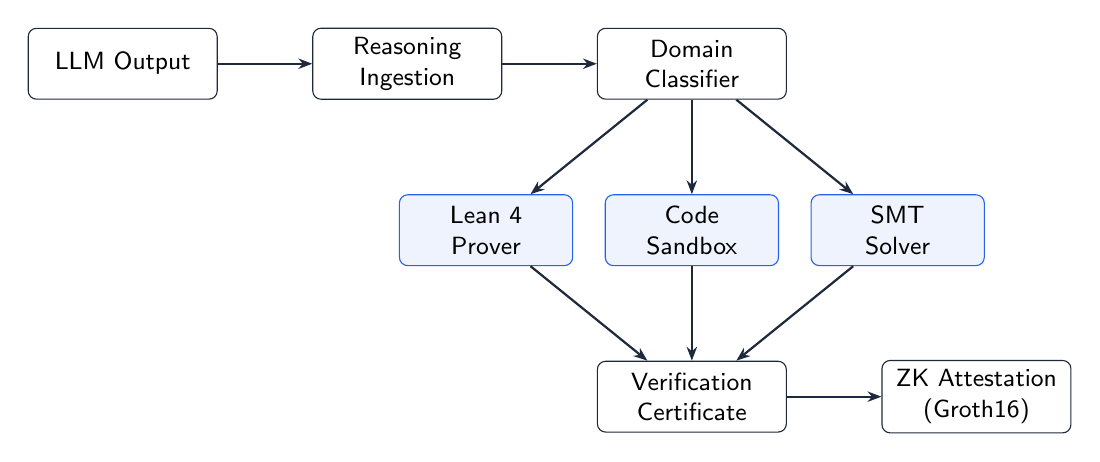
\begin{tikzpicture}[
  node distance=0.6cm and 1.2cm,
  block/.style={
    rectangle, draw=rfdark, fill=white, rounded corners=3pt,
    minimum width=2.4cm, minimum height=0.9cm, align=center,
    font=\small\sffamily
  },
  backend/.style={
    rectangle, draw=rfblue, fill=rfblue!8, rounded corners=3pt,
    minimum width=2.2cm, minimum height=0.9cm, align=center,
    font=\small\sffamily
  },
  arr/.style={-{Stealth[length=5pt]}, thick, color=rfdark},
]
  % Row 1: Ingestion
  \node[block] (input) {LLM Output};
  \node[block, right=of input] (ingest) {Reasoning\\Ingestion};
  \node[block, right=of ingest] (classify) {Domain\\Classifier};

  % Row 2: Backends
  \node[backend, below left=1.2cm and 0.3cm of classify] (lean) {Lean~4\\Prover};
  \node[backend, below=1.2cm of classify] (code) {Code\\Sandbox};
  \node[backend, below right=1.2cm and 0.3cm of classify] (smt) {SMT\\Solver};

  % Row 3: Certificate
  \node[block, below=1.2cm of code] (cert) {Verification\\Certificate};
  \node[block, right=of cert] (zk) {ZK Attestation\\(Groth16)};

  % Arrows
  \draw[arr] (input) -- (ingest);
  \draw[arr] (ingest) -- (classify);
  \draw[arr] (classify) -- (lean);
  \draw[arr] (classify) -- (code);
  \draw[arr] (classify) -- (smt);
  \draw[arr] (lean) -- (cert);
  \draw[arr] (code) -- (cert);
  \draw[arr] (smt) -- (cert);
  \draw[arr] (cert) -- (zk);
\end{tikzpicture}
\caption{ReasonForge verification pipeline.  Structured LLM outputs are
  classified by domain and routed to the appropriate verification
  backend.  Results are aggregated into a verification certificate,
  optionally wrapped in a Groth16 zero-knowledge proof.}
\label{fig:pipeline}
\end{figure}

\subsection{Reasoning Ingestion Layer}
\label{sec:ingestion}

The system accepts structured reasoning chains conforming to the
\texttt{ReasoningTrace} schema---a JSON representation of a multi-step
inference process produced by any LLM or agent framework.  Each trace
encodes: (i) a sequence of labelled reasoning steps, (ii)~the domain
classification of each step (mathematical, code, or logical), (iii)
confidence scores output by the producing model, and (iv) optional
evidence citations.

\begin{lstlisting}[language={},caption={ReasoningTrace input schema.},
  label=lst:trace]
{ "trace_id": "uuid-v4",
  "model": "model-identifier",
  "task": "task description",
  "steps": [
    { "step_id": 1,
      "domain": "mathematical | code | logical",
      "content": "step text",
      "confidence": 0.0--1.0,
      "evidence": ["citation_1", ...] }
  ],
  "conclusion": "final claim" }
\end{lstlisting}

\subsection{Translation and Formalisation Engine}
\label{sec:translation}

Each reasoning step is routed to a domain-appropriate formalisation
module.  The translation process is the technically central component of
ReasonForge: converting free-form natural language reasoning into
representations that admit mechanical verification.

\paragraph{Mathematical Steps $\rightarrow$ Lean~4.}
Mathematical reasoning steps are translated into Lean~4 proof terms using
an autoformalization module.  The produced proof term is submitted to the
Lean~4 type checker; successful type-checking constitutes formal proof of
the step's validity.  Failed type-checking produces a structured error
report identifying the unsound assumption or invalid inference.

\paragraph{Code Logic Steps $\rightarrow$ Property-Based Testing.}
Reasoning steps that make claims about code behaviour are translated into
executable property specifications using property-based testing
frameworks~\citep{hypothesis2019}.  Claims of the form ``function $f$
satisfies property $P$ for all inputs in domain $D$'' are encoded as
typed property tests and executed against a sandboxed evaluation
environment.  Counterexamples produced by the test runner constitute
verification failures with machine-readable witnesses.

\paragraph{Logical Arguments $\rightarrow$ SMT Solvers.}
Logical argument steps are translated into first-order logic formulas
over appropriate theories and submitted to Z3 or CVC5.  The solver either
confirms validity (UNSAT on the negation), returns a satisfying
assignment demonstrating a counterexample (SAT), or times out (UNKNOWN).

\subsection{Code Verification Pipeline}
\label{sec:codeverify}

As the first production instantiation of the general verification
architecture, we have implemented a complete pipeline for verifying
AI-generated Python code.  This pipeline operates independently of the
translation engine and provides end-to-end verification from raw source
code to a scored verification report.  \Cref{fig:codepipeline} shows the
data flow.

\begin{figure}[t]
\centering
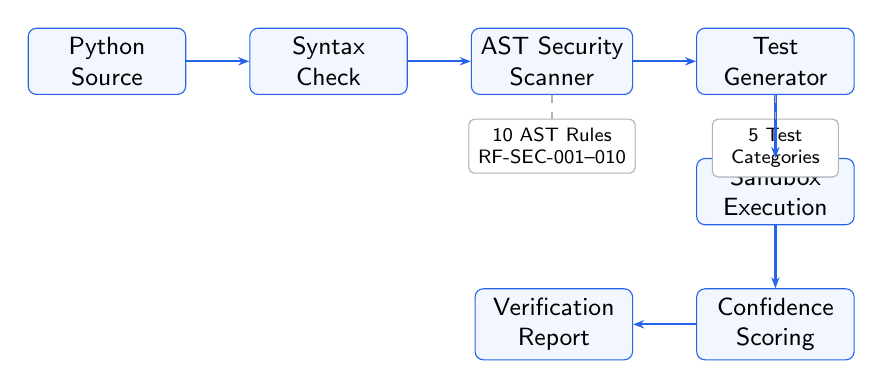
\begin{tikzpicture}[
  node distance=0.4cm and 0.8cm,
  stage/.style={
    rectangle, draw=rfblue, fill=rfblue!6, rounded corners=3pt,
    minimum width=2.0cm, minimum height=0.8cm, align=center,
    font=\small\sffamily
  },
  detail/.style={
    rectangle, draw=gray!60, fill=white, rounded corners=2pt,
    minimum width=1.6cm, minimum height=0.6cm, align=center,
    font=\scriptsize\sffamily
  },
  arr/.style={-{Stealth[length=4pt]}, thick, color=rfblue},
]
  % Pipeline stages
  \node[stage] (src) {Python\\Source};
  \node[stage, right=of src] (syn) {Syntax\\Check};
  \node[stage, right=of syn] (sec) {AST Security\\Scanner};
  \node[stage, right=of sec] (gen) {Test\\Generator};
  \node[stage, below=0.8cm of gen] (exec) {Sandbox\\Execution};
  \node[stage, below=0.8cm of exec] (score) {Confidence\\Scoring};
  \node[stage, left=of score] (report) {Verification\\Report};

  % Detail nodes
  \node[detail, below=0.3cm of sec] (rules) {10 AST Rules\\RF-SEC-001--010};
  \node[detail, below=0.3cm of gen] (cats) {5 Test\\Categories};

  % Arrows
  \draw[arr] (src) -- (syn);
  \draw[arr] (syn) -- (sec);
  \draw[arr] (sec) -- (gen);
  \draw[arr] (gen) -- (exec);
  \draw[arr] (exec) -- (score);
  \draw[arr] (score) -- (report);

  % Detail connections
  \draw[gray!60, dashed] (sec) -- (rules);
  \draw[gray!60, dashed] (gen) -- (cats);
\end{tikzpicture}
\caption{Code verification pipeline.  AI-generated Python source flows
  through syntax checking, AST-based security scanning (10 detection
  rules), static-analysis test generation (5 test categories),
  subprocess-sandboxed pytest execution, and composite confidence
  scoring.}
\label{fig:codepipeline}
\end{figure}

\subsubsection{Sandbox Executor}

The \texttt{SandboxExecutor} runs untrusted Python code in an isolated
subprocess with strict resource limits.  Before execution, a
meta-path import hook is prepended to the code that blocks 10 dangerous
modules (\texttt{os}, \texttt{sys}, \texttt{subprocess},
\texttt{shutil}, \texttt{socket}, \texttt{ctypes}, \texttt{importlib},
\texttt{pathlib}, \texttt{signal}, \texttt{multiprocessing}).  Any
attempt to import a blocked module raises an \texttt{ImportError} with a
descriptive message.  The executor enforces wall-clock timeouts via
subprocess termination and captures stdout, stderr, exit code, and
elapsed time.

\subsubsection{AST-Based Security Scanner}

The \texttt{SecurityScanner} performs static analysis by walking the
Python abstract syntax tree (AST) and applying 10 detection rules:

\begin{table}[h]
\centering
\small
\begin{tabular}{@{}llll@{}}
\toprule
\textbf{Rule ID} & \textbf{Severity} & \textbf{Detects} \\
\midrule
RF-SEC-001 & Critical & \texttt{eval()}/\texttt{exec()} calls \\
RF-SEC-002 & Critical & \texttt{\_\_import\_\_()} calls \\
RF-SEC-003 & High     & Dangerous module imports \\
RF-SEC-004 & High     & \texttt{getattr}/\texttt{setattr} on modules \\
RF-SEC-005 & High     & \texttt{compile()} calls \\
RF-SEC-006 & Medium   & \texttt{open()} without context manager \\
RF-SEC-007 & Low      & Bare \texttt{except} clauses \\
RF-SEC-008 & High     & \texttt{pickle.loads()} deserialisation \\
RF-SEC-009 & Medium   & Hardcoded passwords/secrets \\
RF-SEC-010 & Medium   & Shell injection patterns \\
\bottomrule
\end{tabular}
\caption{Security scanner detection rules.}
\label{tab:secrules}
\end{table}

Each detected vulnerability includes the rule ID, severity level, line
number, category, and a human-readable description.  The scanner assigns
an overall risk level (safe, low, medium, high, or critical) based on the
highest-severity issue found.

\subsubsection{Automated Test Generator}

The \texttt{TestGenerator} produces runnable pytest test suites from
static analysis of function signatures---without requiring an LLM or
external API.  It extracts function signatures (name, parameters, type
annotations, return types, docstrings) via AST parsing and generates five
categories of tests:

\begin{enumerate}[nosep]
  \item \textbf{Callable tests:} Verify the function can be invoked with
    default-typed arguments without raising.
  \item \textbf{Type-check tests:} When return-type annotations are
    present, assert that the return value is an instance of the declared
    type.
  \item \textbf{None-input tests:} Pass \texttt{None} for each parameter
    to check robustness.
  \item \textbf{Docstring example tests:} Parse \texttt{>>>} examples
    from docstrings and assert expected outputs.
  \item \textbf{Edge-case tests:} Generate boundary values for annotated
    types (e.g., $0$, $-1$, empty string for \texttt{int}/\texttt{str}).
\end{enumerate}

\subsubsection{Confidence Scoring}

Each verification report carries a composite confidence score computed as
a weighted sum:

\begin{equation}
  C = w_s \cdot S + w_{\text{sec}} \cdot \text{Sec} + w_t \cdot T
  \label{eq:confidence}
\end{equation}

\noindent where $S \in \{0, 1\}$ is the syntax validity indicator,
$\text{Sec} \in [0, 1]$ is the security score mapped from the risk level
(safe $\mapsto$ 1.0, low $\mapsto$ 0.8, medium $\mapsto$ 0.5, high
$\mapsto$ 0.2, critical $\mapsto$ 0.0), $T \in [0, 1]$ is the test pass
rate, and the weights are $w_s = 0.2$, $w_{\text{sec}} = 0.3$,
$w_t = 0.5$.  The verdict is \textsc{passed} when syntax is valid,
security risk is not critical or high, and $T \geq 0.8$.

\subsection{Verification Certificate}
\label{sec:certificate}

Upon completion of verification across all steps, the system produces a
\texttt{VerificationCertificate}---a structured attestation recording the
verification result for each step, the backend used, any counterexamples
produced, and a cryptographic hash of the input trace binding the
certificate to the specific reasoning chain it attests.

\begin{lstlisting}[language={},caption={VerificationCertificate schema.},
  label=lst:cert]
{ "cert_id": "sha256(...)",
  "trace_hash": "sha256(trace)",
  "timestamp": "ISO-8601",
  "steps": [
    { "step_id": 1,
      "backend": "lean4 | property_test | smt",
      "result": "VERIFIED | FAILED | UNKNOWN",
      "witness": "counterexample or proof term",
      "latency_ms": 142 }
  ],
  "overall": "VERIFIED | PARTIAL | FAILED",
  "zk_proof": "groth16 proof bytes" }
\end{lstlisting}

\subsection{Zero-Knowledge Attestation}
\label{sec:zk}

For enterprise deployments where the reasoning content, model identity,
or input data cannot be disclosed, ReasonForge generates a Groth16
zk-SNARK~\citep{groth2016size} over the verification certificate.  The
proof is generated using a 153-line circom
circuit~\citep{circom2022} compiled to R1CS and proved via
snarkjs~\citep{snarkjs2022}.

\paragraph{Circuit design.}
The \texttt{CertificateVerifier} circuit (\Cref{fig:circuit}) accepts
public inputs (task hash as 8$\times$32-bit limbs, overall verdict,
total steps, verified steps, timestamp) and private inputs (an array of
20 binary step verdicts).  It enforces six constraint classes:

\begin{enumerate}[nosep]
  \item \textbf{Binary constraints:} Each \texttt{step\_verdicts[i]}
    satisfies $x \cdot (1 - x) = 0$.
  \item \textbf{Sum constraint:}
    $\sum_{i=0}^{19} \texttt{step\_verdicts}[i] = \texttt{verified\_steps}$.
  \item \textbf{Verdict consistency:} The \texttt{overall\_verdict}
    follows deterministically from the step counts:
    $\texttt{VERIFIED}$ iff all steps pass and total $> 0$;
    $\texttt{PARTIALLY\_VERIFIED}$ iff some but not all pass;
    $\texttt{FAILED}$ iff zero steps pass.
  \item \textbf{Non-zero witnesses:} Auxiliary inverse signals
    (\texttt{total\_steps\_inv}, \texttt{verified\_steps\_inv},
    \texttt{diff\_inv}) enforce the non-zero checks needed for verdict
    determination.
  \item \textbf{Range checks:} Each task hash limb is decomposed into
    32~bits with binary constraints, ensuring limb values are in
    $[0, 2^{32} - 1]$.
  \item \textbf{Indicator exclusivity:} Exactly one of
    \texttt{is\_all\_verified}, \texttt{is\_partial},
    \texttt{is\_failed} is~1.
\end{enumerate}

The circuit enables the following attestation statement: ``\emph{A
reasoning trace with task hash $H$ was submitted to the ReasonForge
verification pipeline and received verdict $V$ with $k$ of $n$ steps
verified}''---without revealing the individual step verdicts or the
source code.  The proof is constant-size (128--256 bytes for Groth16) and
verifiable in $O(1)$ time by any party holding the verification key.

\begin{figure}[t]
\centering
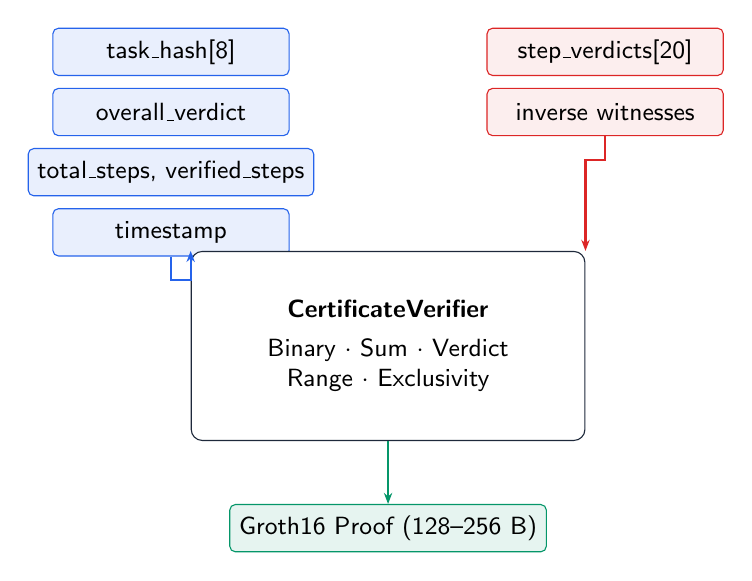
\begin{tikzpicture}[
  node distance=0.5cm,
  pub/.style={
    rectangle, draw=rfblue, fill=rfblue!10, rounded corners=2pt,
    minimum width=3cm, minimum height=0.6cm, align=center,
    font=\small\sffamily
  },
  priv/.style={
    rectangle, draw=rfred, fill=rfred!8, rounded corners=2pt,
    minimum width=3cm, minimum height=0.6cm, align=center,
    font=\small\sffamily
  },
  circ/.style={
    rectangle, draw=rfdark, fill=white, rounded corners=4pt,
    minimum width=5cm, minimum height=2.4cm, align=center,
    font=\small\sffamily
  },
  output/.style={
    rectangle, draw=rfgreen, fill=rfgreen!10, rounded corners=2pt,
    minimum width=3cm, minimum height=0.6cm, align=center,
    font=\small\sffamily
  },
  arr/.style={-{Stealth[length=4pt]}, thick},
]
  % Public inputs
  \node[pub] (ph) {task\_hash[8]};
  \node[pub, below=0.15cm of ph] (pv) {overall\_verdict};
  \node[pub, below=0.15cm of pv] (pts) {total\_steps, verified\_steps};
  \node[pub, below=0.15cm of pts] (pt) {timestamp};

  % Private inputs
  \node[priv, right=2.5cm of ph] (sv) {step\_verdicts[20]};
  \node[priv, below=0.15cm of sv] (inv) {inverse witnesses};

  % Circuit
  \node[circ, below=1.0cm of $(pt)!0.5!(inv)$] (circuit) {%
    \textbf{CertificateVerifier}\\[3pt]
    Binary $\cdot$ Sum $\cdot$ Verdict\\
    Range $\cdot$ Exclusivity};

  % Output
  \node[output, below=0.8cm of circuit] (proof) {Groth16 Proof (128--256 B)};

  % Arrows
  \draw[arr, rfblue] (pt.south) -- ++(0,-0.3) -| (circuit.north west);
  \draw[arr, rfred] (inv.south) -- ++(0,-0.3) -| (circuit.north east);
  \draw[arr, rfgreen] (circuit) -- (proof);
\end{tikzpicture}
\caption{ZK certificate circuit.  Public inputs (blue) and private step
  verdicts (red) are constrained by the CertificateVerifier circuit to
  produce a constant-size Groth16 proof (green).}
\label{fig:circuit}
\end{figure}

% ======================================================================
\section{Decentralised Verification Network}
\label{sec:network}
% ======================================================================

While ReasonForge can operate as a centralised service, its full design
includes a decentralised verification network in which independent
validator nodes compete to produce accurate verification results.
\Cref{fig:network} illustrates the network topology.

\begin{figure}[t]
\centering
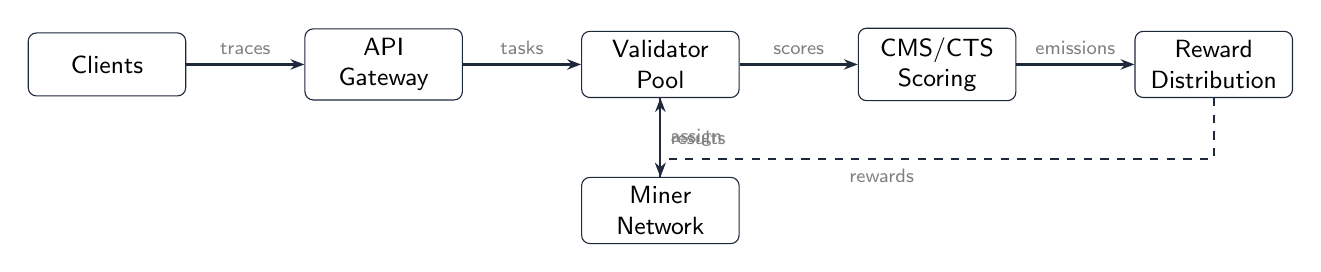
\begin{tikzpicture}[
  node distance=1.0cm and 1.5cm,
  role/.style={
    rectangle, draw=rfdark, fill=white, rounded corners=3pt,
    minimum width=2.0cm, minimum height=0.8cm, align=center,
    font=\small\sffamily
  },
  arr/.style={-{Stealth[length=5pt]}, thick, color=rfdark},
  lbl/.style={font=\scriptsize\sffamily, color=gray},
]
  \node[role] (client) {Clients};
  \node[role, right=of client] (api) {API\\Gateway};
  \node[role, right=of api] (val) {Validator\\Pool};
  \node[role, below=of val] (miner) {Miner\\Network};
  \node[role, right=of val] (score) {CMS/CTS\\Scoring};
  \node[role, right=of score] (reward) {Reward\\Distribution};

  \draw[arr] (client) -- node[above,lbl]{traces} (api);
  \draw[arr] (api) -- node[above,lbl]{tasks} (val);
  \draw[arr] (val) -- node[right,lbl]{assign} (miner);
  \draw[arr] (miner) -- node[right,lbl]{results} (val);
  \draw[arr] (val) -- node[above,lbl]{scores} (score);
  \draw[arr] (score) -- node[above,lbl]{emissions} (reward);
  \draw[arr, dashed] (reward) -- ++(0,-1.2) -| node[below,lbl,pos=0.3]{rewards} (miner);
\end{tikzpicture}
\caption{Decentralised verification network.  Clients submit reasoning
  traces via the API.  Validators assign tasks to miners, score
  submissions using CMS/CTS, and distribute rewards proportionally.}
\label{fig:network}
\end{figure}

\subsection{Network Roles}

\textbf{Miners} are nodes that receive reasoning traces, execute the
formalisation and verification pipeline, and submit verification results
with structured outputs.  \textbf{Validators} are nodes that score miner
submissions using automated objective checks and stake-weighted
consensus.  \textbf{Clients} submit reasoning traces via the API and
consume verification certificates.

\subsection{Composite Miner Score (CMS)}

Each miner $m$ receives a Composite Miner Score for each task $t$,
computed as a weighted sum across four performance dimensions:

\begin{equation}
  \text{CMS}(m, t) = w_q \cdot Q(m,t) + w_a \cdot A(m,t)
    + w_n \cdot N(m,t) + w_e \cdot \text{Eff}(m,t)
  \label{eq:cms}
\end{equation}

\noindent where $Q$ is verification quality (correctness of formal
representations), $A$ is argument completeness (step coverage), $N$ is
novelty (distance from prior submissions), and $\text{Eff}$ is
computational efficiency (latency relative to difficulty).  Weights
$w_q = 0.45$, $w_a = 0.30$, $w_n = 0.15$, $w_e = 0.10$ reflect the
primacy of correctness.

The epoch-level miner score aggregates across all tasks assigned in epoch
$\mathcal{T}$, weighted by task difficulty $D(t)$:

\begin{equation}
  S_{\text{epoch}}(m) = \frac{1}{|\mathcal{T}_m|}
    \sum_{t \in \mathcal{T}_m} \text{CMS}(m, t) \cdot D(t)
  \label{eq:sepoch}
\end{equation}

\subsection{Composite Translation Score (CTS)}

For the translation and formalisation workflow, miners are additionally
scored on translation quality via the Composite Translation Score:

\begin{equation}
  \text{CTS}(m, t) = w_c \cdot C_{\text{comp}}(m,t)
    + w_r \cdot C_{\text{corr}}(m,t)
    + w_p \cdot C_{\text{cmpl}}(m,t)
    + w_f \cdot C_{\text{eff}}(m,t)
  \label{eq:cts}
\end{equation}

\noindent where $C_{\text{comp}}$ measures whether the translated formal
representation compiles in the target system (Lean~4/Z3/Python),
$C_{\text{corr}}$ measures semantic correctness against ground-truth when
available, $C_{\text{cmpl}}$ measures completeness of the translation
(fraction of reasoning steps successfully formalised), and
$C_{\text{eff}}$ penalises excessive translation latency.  Weights
$w_c = 0.40$, $w_r = 0.25$, $w_p = 0.20$, $w_f = 0.15$ prioritise
compilation success as the minimum quality bar.

\subsection{Persistent Excellence Bonus (PEB)}

To incentivise sustained high performance rather than one-shot
optimisation, the top-$K$ miners ($K = 10$) receive a Persistent
Excellence Bonus:

\begin{equation}
  \text{PEB}(m) = \alpha \cdot \frac{1}{\text{rank}(m)}
    \cdot \text{streak}(m)^{0.5}
  \label{eq:peb}
\end{equation}

\noindent where $\alpha = 0.15$ is a global scaling factor.  The
sub-linear growth of the streak term prevents unbounded bonus
accumulation while still rewarding consistency.

\subsection{Breakthrough Discovery Multiplier}

When a miner produces a valid formal proof for a previously unverified
claim class---i.e., the verification backend returns PROVED for the first
time on a novel problem variant---a one-time multiplier is applied:

\begin{equation}
  \text{CMS}_{\text{break}}(m, t) = \text{CMS}(m, t) \cdot \beta,
  \quad \beta = 2.0
  \label{eq:breakthrough}
\end{equation}

\subsection{Validator Accuracy Score (VAS)}

Validators are rewarded for accurate, honest scoring.  The Validator
Accuracy Score measures deviation from consensus:

\begin{equation}
  \text{VAS}(v) = 1 - \frac{1}{|\mathcal{T}_v|}
    \sum_{t \in \mathcal{T}_v}
    \frac{|\text{score}_v(m,t) - \text{score}_{\text{consensus}}(m,t)|}
         {\text{max\_dev}}
  \label{eq:vas}
\end{equation}

\subsection{Incentive Alignment}

The mechanism is designed to satisfy four incentive properties required
for a robust proof-of-intelligence protocol:

\begin{enumerate}[nosep]
  \item \textbf{Monotonicity.} Higher CMS strictly yields greater
    reward.  No threshold effects that could incentivise strategic
    sandbagging.
  \item \textbf{Process supervision.} Scoring every reasoning step
    eliminates the dominant strategy of guessing final answers without
    genuine verification effort.
  \item \textbf{Difficulty weighting.} $D(t)$ prevents mining of
    trivially easy tasks---harder verification problems yield
    proportionally greater reward.
  \item \textbf{Validator honesty as dominant strategy.} Validators who
    deviate from accurate scoring reduce their own VAS and face
    progressive quadratic slashing (\Cref{sec:adversarial}), making
    honest evaluation strictly dominant under rational self-interest.
\end{enumerate}

\noindent We note that these are design-level arguments, not formal
game-theoretic proofs.  A full equilibrium analysis under adaptive
adversaries is planned as future work.

\subsection{Adversarial Resistance}
\label{sec:adversarial}

\paragraph{Trap Problem Injection.}
15\% of tasks in each miner's queue are trap problems---tasks with
verified ground-truth solutions drawn from a curated benchmark suite.
Miners cannot distinguish trap from non-trap tasks ex-ante.  If a miner's
trap score falls below threshold $\theta_{\text{trap}} = 0.3$, a
multiplicative penalty is applied:

\begin{equation}
  S_{\text{epoch}}(m) \leftarrow S_{\text{epoch}}(m)
    \cdot \max\!\left(0,\,
    \frac{\text{trap\_score}(m)}{\theta_{\text{trap}}}\right)
  \label{eq:trap}
\end{equation}

\paragraph{Blind Evaluation Protocol.}
Miner identities are replaced with cryptographic hashes before validator
assignment.  Each submission is evaluated by a minimum of three
independently selected validators.  Submissions are committed via hash
before content is revealed, preventing post-hoc modification.

\paragraph{Validator Quadratic Slashing.}
Validators whose VAS consistently falls below threshold
$\theta_{\text{slash}}$ face progressive quadratic slashing on staked
collateral:

\begin{equation}
  \text{slash}(v) = \gamma \cdot \text{stake}(v)
    \cdot \max\!\left(0,\,
    \theta_{\text{slash}} - \text{VAS}_{\text{avg}}(v, 7\text{d})
    \right)^{2}
  \label{eq:slash}
\end{equation}

\paragraph{Similarity Penalty.}
All miner submissions are checked against a rolling similarity index.
Submissions with cosine similarity $> 0.95$ to any submission from the
past 30 epochs receive a $0.5\times$ multiplier on their CMS,
discouraging plagiarism and incentivising genuine novel verification work.

% ======================================================================
\section{Experimental Evaluation}
\label{sec:evaluation}
% ======================================================================

We evaluate the ReasonForge implementation across five dimensions:
system scale, code verification accuracy, security scanner coverage,
sandbox isolation effectiveness, and end-to-end pipeline performance.
All experiments were conducted on a Windows~10 machine with Python~3.9.13.

\subsection{System Scale}

The complete implementation comprises 37 Python source files totalling
7{,}418 lines of code across six packages (\texttt{codeverify},
\texttt{certificates}, \texttt{translation}, \texttt{verification},
\texttt{protocol}, and \texttt{engine}), plus a 153-line circom ZK
circuit.  The test suite consists of 10 test files with 4{,}233 lines,
providing 316 test cases.  Of these, 310 pass unconditionally and 6
require external ZK tooling (circom compiler and snarkjs) and are
automatically skipped when those tools are not installed.

\begin{table}[h]
\centering
\small
\begin{tabular}{@{}lrr@{}}
\toprule
\textbf{Package} & \textbf{Source Files} & \textbf{Lines} \\
\midrule
\texttt{codeverify}    & 8  & 2{,}627 \\
\texttt{certificates}  & 7  & 1{,}260 \\
\texttt{translation}   & 5  &   469 \\
\texttt{verification}  & 7  &   733 \\
Core modules           & 10 & 2{,}329 \\
\midrule
\textbf{Total}         & 37 & 7{,}418 \\
\bottomrule
\end{tabular}
\quad
\begin{tabular}{@{}lrr@{}}
\toprule
\textbf{Test File} & \textbf{Tests} & \textbf{Lines} \\
\midrule
Certificates        & 77  & 1{,}239 \\
Code verify (unit)  & 38  &   450 \\
Code verify (integ) &  7  &   197 \\
Engine              & 40  &   410 \\
Proof layer sim     & 24  &   302 \\
Protocol            & 28  &   371 \\
Simulator           & 10  &   179 \\
Translation         & 32  &   384 \\
Types               & 17  &   164 \\
Verification        & 43  &   537 \\
\midrule
\textbf{Total}      & 316 & 4{,}233 \\
\bottomrule
\end{tabular}
\caption{Implementation scale: source code (left) and test suite
  (right).}
\label{tab:scale}
\end{table}

\subsection{HumanEval Benchmark Evaluation}

To evaluate the code verification pipeline on a standardised corpus of
AI-quality Python code, we ran all 164 canonical solutions from the
OpenAI HumanEval benchmark~\citep{humaneval2021} through the full
\texttt{VerificationPipeline}.  \Cref{tab:humaneval} summarises the
results.

\begin{table}[h]
\centering
\small
\begin{tabular}{@{}lr@{}}
\toprule
\textbf{Metric} & \textbf{Value} \\
\midrule
Total problems evaluated  & 164 \\
Pipeline errors           & 0 \\
Verdict: \textsc{passed}  & 55 (33.5\%) \\
Verdict: \textsc{failed}  & 109 (66.5\%) \\
Syntax pass rate          & 100.0\% \\
Security: safe            & 161 (98.2\%) \\
Security: low             & 2 (1.2\%) \\
Security: critical        & 1 (0.6\%) \\
Mean tests generated/func & 4.3 \\
Mean test pass rate       & 63.9\% \\
Mean confidence score     & 0.817 \\
\midrule
Median latency            & 2{,}230\,ms \\
Mean latency              & 3{,}612\,ms \\
P95 latency               & 13{,}317\,ms \\
\bottomrule
\end{tabular}
\caption{ReasonForge pipeline results on the HumanEval benchmark
  (164 canonical solutions).}
\label{tab:humaneval}
\end{table}

\paragraph{Syntax and security.}
All 164 functions pass syntax validation (100\%).  The security scanner
correctly classifies 161 functions (98.2\%) as safe, flags 2 functions
for bare \texttt{except} clauses (RF-SEC-007, low severity), and
identifies 1 function containing \texttt{eval()} (RF-SEC-001, critical
severity).  Zero false positives were observed for dangerous-import
detection.

\paragraph{Verification verdicts.}
55 functions (33.5\%) receive a \textsc{passed} verdict, meaning they
satisfy all three criteria: valid syntax, security risk below ``high,''
and auto-generated test pass rate $\geq 80\%$.  The remaining 109
functions (66.5\%) are classified as \textsc{failed}, with the primary
failure reason being test pass rates below the 80\% threshold.

\paragraph{Analysis of failures.}
The 66.5\% failure rate is a deliberate consequence of the pipeline's
design: the test generator produces robustness tests---including
\texttt{None}-input tests, edge-case tests with boundary values, and
type-check tests---that most HumanEval solutions do not handle.  HumanEval
canonical solutions assume well-typed inputs and do not include defensive
programming for \texttt{None} or out-of-domain values.  A function like
\texttt{def add(a:~int, b:~int) -> int: return a + b} is \emph{correct}
but not \emph{robust}: it raises \texttt{TypeError} when passed
\texttt{None}.  The pipeline identifies this as a verification failure
because the function's behaviour is undefined outside its declared domain.

This result demonstrates that ReasonForge measures \textbf{robustness}
beyond \textbf{correctness}.  Functions that pass ReasonForge verification
are not merely correct implementations---they are defensively programmed
against malformed or adversarial inputs.  The mean confidence score of
0.817 across all 164 functions reflects the high syntax and security
scores ($\sim$1.0 each) moderated by the lower test pass rate (63.9\%).

\paragraph{Latency.}
The median verification latency of 2.2~seconds per function is dominated
by subprocess-sandboxed pytest execution.  The P95 latency of 13.3~seconds
corresponds to functions with larger generated test suites or complex
execution paths.  Syntax checking and AST security scanning complete in
under 10\,ms per function.

\subsection{Security Scanner Coverage}

All 10 AST-based detection rules were individually validated with
targeted test samples (38 unit tests).  Each rule correctly identifies
its vulnerability class, assigns the expected severity level, and reports
the correct line number.  On the HumanEval corpus, the scanner produced
zero false positives for dangerous-import detection (rules RF-SEC-003
through RF-SEC-005) and correctly identified the single function
containing \texttt{eval()} (RF-SEC-001).  The scanner handles
syntactically invalid input gracefully by returning a ``critical'' risk
assessment with a \texttt{RF-SEC-SYNTAX} pseudo-rule.

\subsection{End-to-End Pipeline Performance}

The full unit test suite of 316 tests executes in approximately
12~seconds.  The HumanEval benchmark of 164 functions completes in
approximately 10~minutes (mean 3.6\,s per function).  The pipeline
produces deterministic code hashes for identical inputs and distinct
hashes for different inputs, ensuring certificate uniqueness.  The
certificate round-trip---pipeline verification $\rightarrow$ report
$\rightarrow$ ZK certificate creation $\rightarrow$ registry
registration $\rightarrow$ look-up $\rightarrow$
verification---completes successfully for all test scenarios.

% ======================================================================
\section{Applications and Use Cases}
\label{sec:applications}
% ======================================================================

\subsection{Autonomous Code Generation}

AI code generation systems (Copilot, Cursor, Codex) produce code that is
deployed without formal verification of correctness or safety.
ReasonForge's code verification pipeline can be integrated as a
post-generation gate: AI-generated Python code is automatically scanned
for security vulnerabilities, tested via generated test suites, and
issued a verification certificate with a confidence score.  A VS Code
extension prototype demonstrates this workflow, enabling developers to
verify AI-generated code with a single command.

\subsection{Medical AI}

Diagnostic AI systems that chain clinical observations through
differential reasoning to conclusions can submit each reasoning step to
ReasonForge for verification against established clinical logic
encodings.  A verification certificate accompanying an AI diagnostic
recommendation allows clinicians and regulators to audit not just the
recommendation but the logical path that produced it---without requiring
access to model weights or proprietary training data.

\subsection{Financial Risk Modelling}

Quantitative models that produce risk assessments through multi-step
analytical chains---portfolio stress tests, credit scoring pipelines,
derivative pricing models---can attest verification of each analytical
step to regulators via ZK certificates.  This satisfies emerging Model
Risk Management (MRM) guidance requiring explainable audit trails for
AI-driven financial decisions.

\subsection{Legal Reasoning Systems}

Legal AI systems constructing argument chains---statute interpretation,
precedent application, contract clause analysis---can produce step-level
verification against formal logic encodings of legal rules.  Verification
certificates provide machine-readable attestations of argument structure
validity that complement human legal review.

% ======================================================================
\section{Limitations and Open Problems}
\label{sec:limitations}
% ======================================================================

ReasonForge inherits the fundamental scope limitation of formal
verification: it can only verify claims that can be expressed in the
target formal language.  Empirical claims, value judgements, and claims
requiring world knowledge beyond encoded axioms fall outside the
mechanically verifiable scope.  The system explicitly marks such steps as
\textsc{unknown} rather than \textsc{verified}.  Extending the system to
empirical claims---via retrieval-augmented claim verification against
curated knowledge bases such as Wikidata, PubMed, and established
scientific databases---is a planned future direction.

The quality of verification is bounded by the quality of translation from
natural language to formal representations.  Translation errors---producing
a formally valid proof of a claim that does not accurately capture the
intended natural language statement---represent the primary failure mode.
This is an active area of research in autoformalization and is not unique
to ReasonForge.

The current ZK implementation uses Groth16 proofs, which require a
trusted setup ceremony.  The circuit-specific setup produces a proving
key and verification key that must be generated honestly; a compromised
setup allows forging proofs.  Migration to a transparent proof system
(e.g., STARK or PLONK with a universal SRS) would eliminate this trust
assumption at the cost of larger proof sizes.

The incentive alignment arguments in \Cref{sec:network} are design-level
arguments, not formal game-theoretic proofs.  A complete equilibrium
analysis under adaptive adversaries, including collusion resistance
bounds and Sybil attack thresholds, is an open problem.

Additional open problems include: (i)~improving translation fidelity for
advanced mathematical reasoning beyond undergraduate-level mathematics;
(ii)~reducing verification latency to support real-time reasoning
pipelines; (iii)~formal security analysis of the ZK attestation scheme
under adaptive adversaries; and (iv)~extending the code verification
pipeline to additional programming languages beyond Python.

% ======================================================================
\section{Conclusion}
\label{sec:conclusion}
% ======================================================================

We have presented ReasonForge, a protocol and system architecture for the
mechanical verification of multi-step AI reasoning chains.  The system
translates structured LLM outputs into formally verifiable
representations across three verification backends, produces
machine-checkable certificates, and encapsulates these certificates in
Groth16 zero-knowledge proofs for privacy-preserving compliance
attestation.

The production code-verification pipeline---comprising AST-based security
scanning with 10 detection rules, automated test generation from static
analysis, and subprocess-sandboxed pytest execution---demonstrates the
architecture's viability as a concrete, deployable system.  The
accompanying decentralised verification network provides economic
incentive alignment for independent validators through the CMS and CTS
scoring frameworks, with adversarial resistance mechanisms including trap
problem injection, blind evaluation, and quadratic slashing.

The implementation comprises 7{,}418 lines of Python across 37 modules, a
153-line circom ZK circuit, and 316 automated tests.  The complete system
is released as open-source software.

The fundamental argument of this paper is architectural: the AI stack is
missing a trust layer for reasoning.  Output evaluation measures what a
model says.  Process verification measures whether the reasoning that
produced it is sound.  As AI systems move deeper into consequential
domains, the latter becomes the more important property.  ReasonForge is
a step toward making it provable.

\medskip
\noindent The protocol specification, verification backends, ZK circuit,
scoring formulas, and full test suite are open source and available at
\url{https://github.com/UNSPECIFIEDCODER/ReasonForge}.

% ── References ────────────────────────────────────────────────────────────
\bibliography{refs}

\end{document}
